\section{Automatic differentiation}
\label{sec:autom-diff}

\index{automatic~differentiation}\emph{Automatic differentiation}
(\index{AD@see{automatic~differentiation}}AD) studies the following
question: given a program to evaluate a function $f:R^n\ra R$ at a
point of $R^n$, how much does it cost to evaluate the gradient $\nabla
f$ at a point of $R^n$. More generally, one can consider functions
$R^n\ra R^n$ and ask for the evaluation of the Jacobian matrix $J_f$.

\subsection{From automatic differentiation to transposition}
\label{sec:from-autom-diff}
Transposition of linear straight line programs reduces to automatic
differentiation, in fact, if one has a program computing a linear
function $f:R^n\ra R^m$ and a $\ell\in\dual{(R^m)}$,
\begin{equation}
  \label{eq:261}
  \nabla (\ell\circ f) =
  \left(\frac{\partial \ell\circ f}{\partial x_1},\ldots,\frac{\partial \ell\circ f}{\partial x_n}\right) =
  \left(\braket{\dual{f}(\ell)}{\basis{e}_1},\ldots,\braket{\dual{f}(\ell)}{\basis{e}_n}\right)
  \text{,}
\end{equation}
where $(\basis{e}_1,\ldots,\basis{e}_n)$ is the standard basis of
$R^n$. Thus, differentiating the program for $\ell\circ f$ yields the
coordinates of $\dual{f}(\ell)$ on the standard basis of
$\dual{(R^n)}$ as requested.

Automatic differentiation is widely used in numerical computations and
this is why there is an extensive literature on it. In particular the
\index{reverse~mode}\index{automatic~differentiation!reverse~mode}\emph{reverse
  mode} with the
\index{automatic~differentiation!checkpoint~method}\index{checkpoint~method}\emph{checkpoint
  method} of Griewank~\cite{griewank92} implies that automatic
differentiation of functions $R^n\ra R$ can be done with a constant
factor penalty in algebraic time complexity and an $O(\log(n))$
penalty in algebraic space complexity. However, this is still far from
the bounds of Theorem~\ref{th:tellegen-R-algeb}.

Using the method of the
\index{adjoint~code}\index{automatic~differentiation!adjoint~code}{adjoint
  code} with optimizations for linear
instructions~\cite{gilbert+levey+masse91}, it is possible to save even
more and ultimately reduce to the bounds of the transposition
principle. This is not surprising as the adjoint code on linear
programs is exactly the same thing as the transposition of linear
straight line programs we saw in the previous section.

However, automatic differentiation uses a lot of machinery that has
been tailored for non-linear programs. Using it for transposition is
just overkill. Even worse, it is clumsy because automatic
differentiation is built on top of the transposition principle as it
was pointed out by~\cite{gashkov+gashkov05}. To see this we shall
briefly recall how automatic differentiation works on arithmetic
circuits.

\subsection{Differentiation of arithmetic circuits}
\label{sec:diff-arithm-circ}
\pdfmcone{Éric: justement, "arithmetic circuits" implique
  qu'on est dans le monde de la complexité algébrique, non? Il ne me
  semble pas qu'il y ait des travaux précédents à Baur-Strassen qui
  parlent de differentiation ET de circuits arithmétiques.} The first
result on differentiation of arithmetic circuits is due to Baur and
Strassen~\cite{baur+strassen83}. They show that a non-linear
arithmetic circuit that computes a function $f:R^n\ra R$ can be
transformed in a circuit to compute $f$ and $\nabla f$ with a
three-fold increase in size. Gashkov and
Gashkov~\cite{gashkov+gashkov05} interpret their method as a
transformation that yields a circuit to compute $f$ and the
differential $\diff f$ at a point $x$ and $n$ differential inputs
$\diff x_1,\ldots,\diff x_n$; then, an application of the
transposition principle on linearized circuits as in
Section~\ref{sec:multilinear-circuits}, yields the original result of
Baur and Strassen.

Here we describe the transformation of~\cite{gashkov+gashkov05} in a
simplified manner. A complete description can be found
in~\cite{gashkov+gashkov05,sergeev08}.

For simplicity, we consider an arithmetic circuit $C$ over a
non-linear basis $\mathcal{B}$ over $\R$ made exclusively of
everywhere continuously derivable functions (w.r.t the standard metric
of the Euclidean space $\R^n$). We describe a technique to compute the
differential of $\eval_C$ at a point $a\in\R^n$.

\begin{definition}[Differential of a circuit]
  \index{differential~of~a~circuit}\index{arithmetic~circuit!differential}
  Let $C=(V,E,\le,\le_i,\le_o)$ be a circuit over $(\R,\mathcal{B})$
  with $n$ inputs and $m$ outputs and let $a\in\R^n$. For any function
  $f\in\mathcal{B}$, we denote by $J_f$ its Jacobian. 

  The \emph{differential} of $C$ at $a$, denoted by $\diff_a C$, is
  obtained by substituting each $\beta(v)$ with
  \begin{equation}
    \label{eq:derivative}
    \beta'(v)=J_f\left(\eval_{e_1}(a),\ldots,\eval_{e_k}(a)\right)
  \end{equation}
  for any $v\in V$, where $e_1,\ldots,e_k$ are the edges incident to
  $v$.
\end{definition}

\begin{figure}[!ht]
  \centering
  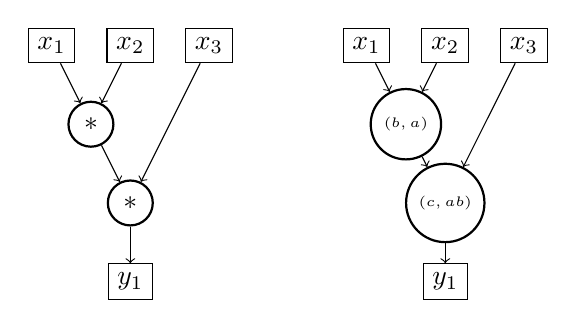
\begin{tikzpicture}
    \tikzstyle{node}=[circle,thick,draw=black,minimum size=4mm]
    \tikzstyle{arg}=[rectangle,thin,draw=black,minimum size=4mm]
    
    \begin{scope}
      \node[arg](in1){$x_1$};
      \node[arg,right of=in1](in2){$x_2$};
      \node[arg,right of=in2](in3){$x_3$};
      \node[node,below of=in1,xshift=5mm](times1){$*$};
      \node[node,below of=times1,xshift=5mm](times2){$*$};
      \node[arg,below of=times2](out){$y_1$};

      \path[->]
      (in1) edge (times1)
      (in2) edge (times1)
      (times1) edge (times2)
      (in3) edge (times2)
      (times2) edge (out);
    \end{scope}

    \begin{scope}[xshift=4cm]
      \node[arg](in1){$\diff x_1$};
      \node[arg,right of=in1](in2){$\diff x_2$};
      \node[arg,right of=in2](in3){$\diff x_3$};
      \node[node,below of=in1,xshift=5mm](times1){\tiny$(b,a)$};
      \node[node,below of=times1,xshift=5mm](times2){\tiny$(c,ab)$};
      \node[arg,below of=times2](out){$\diff y_1$};

      \path[->]
      (in1) edge (times1)
      (in2) edge (times1)
      (times1) edge (times2)
      (in3) edge (times2)
      (times2) edge (out);
    \end{scope}
  \end{tikzpicture}
  \caption{A circuit and its derivative at the point $(a,b,c)$. We
    have replaced multiplication nodes with linear applications
    represented by $1\times2$ matrices.}
  \label{fig:derivative}
\end{figure}


\begin{proposition}
  The differential of a circuit satisfies $\eval_{\diff_aC}=J_{\eval_C}(a)$ for any $a\in\R^n$.
\end{proposition}
\begin{proof}
  Let $e$ be and edge of $C$, we shall denote by $\eval_e$ its
  evaluation as in Definition~\ref{def:eval}, and by $\eval_e'$ the
  evaluation of the corresponding edge in $\diff_a C$.  We prove that
  for any $a\in\R^n$ and for any edge $e$ of $C$, the differential of
  $\eval_e$ at $a$ is $\eval_e'$.  The proof is by induction and
  follows by the chain rule.

  Let $x_1\le_i\cdots\le_ix_n$ be the inputs of $C$, we write
  $f(\lst{x})$ for $f(x_1,\ldots,x_n)$.  Let $v$ be a node, let
  $e_1\le_v\cdots\le_ve_k$ be its input edges and let $e$ be the
  $i$-th output edge. Set $f=\beta(v)$, then by
  \hyperref[def:eval]{definition}
  \begin{equation}
    \label{eq:266}
    \begin{aligned}
      \eval_v &= f \circ (\eval_{e_1},\ldots,\eval_{e_k})\text{,}\\
      \eval_e &= \pi_i\circ\eval_v \text{,}
    \end{aligned}
  \end{equation}
  where $\pi_i$ is the $i$-th projection. Then, the Jacobian matrix of
  $\eval_v$ is
  \begin{equation}
    \label{eq:267}
    J_{\eval_v}(\lst{x}) =
    J_f(\eval_{e_1},\ldots,\eval_{e_k}) J_{(\eval_{e_1},\ldots,\eval_{e_k})} (\lst{x})
    \text{.}
  \end{equation}
  Hence, $\diff_a \eval_v$ is equal to
  \begin{equation}
    \label{eq:268}
    J_{\eval_v}(a)
    \begin{pmatrix}
      \diff_{a} x_1\\\vdots\\\diff_{a} x_n
    \end{pmatrix} =
    \beta'(v)
    \begin{pmatrix}
      \diff_a \eval_{e_1}\\\vdots\\\diff_a \eval_{e_n}
    \end{pmatrix} =
    \beta'(v)\circ (\eval_{e_1}',\ldots,\eval_{e_n}')
    \text{,}
  \end{equation}
  where the last equality follow by induction. By
  \hyperref[def:eval]{definition}, this is the evaluation of $v$ in
  $\diff_{a} C$, and the claim follows by composing with $\pi_i$.
\end{proof}

It is also clear that $\diff_aC$ is defined over a linear basis over
$\R$, thus the \hyperref[th:tellegen]{transposition theorem} applies
to it. In other words we have defined a transformation from circuits
computing derivable functions to linear circuits. 

Also notice that when $C$ is a linear circuit, then simply
$C=\diff_aC$ for any $a$. In this case, Eq.~\eqref{eq:261} amounts to
plug the form $\ell$ at the bottom of $C$, then, transposing
$\diff_aC=C$ and evaluating at $1$ gives the desired coefficients of
$\dual{f}(\ell)$.


\begin{nota}
  The construction of~\cite{gashkov+gashkov05} is more powerful: they
  start from a non-linear circuit $C$ with input nodes
  $x_1,\ldots,x_n$, and they augment it to obtain a non linear circuit
  $C'$ with input nodes $x_1,\ldots,x_n,\diff x_1,\ldots,\diff x_n$;
  this circuit admits a linearization $\ell=\{\diff x_1,\ldots,\diff
  x_n\}$, in the sense of Definition~\ref{def:linearization}, and they
  prove that $C'_\ell=\diff_{\lst{x}} C$. Then, Baur and Strassen's theorem
  follows by considering $\dual{{C'_\ell}}$.
\end{nota}



\subsection{From transposition to automatic differentiation}
\label{sec:from-transp-autom}
The circuit $\diff_a C$ is an important intermediate step to compute
the gradient: any automatic differentiator computes it, either
explicitly or implicitly.

Now $\diff_aC$ can be queried by black-box algorithms to obtain
information about the Jacobian $J_{\eval_C}(a)$. The simplest
application is to compute the directional derivative in $a$ along a
direction $u$: for this task it suffices to evaluate the circuit once,
since $\eval_{\diff_aC}(u)$ is the desired value. Computing the
derivative along $n$ linearly independent directions yields the whole
Jacobian matrix and this roughly corresponds to the
\index{direct~mode}\index{automatic~differentiation!direct~mode}\emph{direct
  mode} in automatic differentiation.

\begin{remark}
  To be more precise, direct mode automatic differentiation constructs
  $\diff_aC$ and evaluates the $n$ directions in parallel, thus
  avoiding the need to store the whole circuit in memory. This is a
  great advantage for iterative code, where $C$ can be represented
  compactly by a for loop, but $\diff_a C$ needs the loop to be
  unrolled.
\end{remark}

When the circuit has many inputs but only one output, there is a more
convenient way to get $\nabla \eval_C$ with only one black-box query:
$\diff_aC$ computes a linear form whose coefficients are exactly the
coefficients of the gradient, thus the dual circuit
$\dual{(\diff_aC)}$ computes the transposed form. The single query
$\eval_{\dual{(\diff_aC)}}(1)$ yields this vector. This is exactly
what is called ``reverse mode'' in automatic differentiation. 

\begin{remark}
  Unlike the direct mode, reverse mode cannot compute
  $\dual{(\diff_aC)}$ and evaluate on a direction in parallel. One
  solution is to store the whole $\diff_aC$ in memory, but this object
  may be too large. The checkpoint method of
  Griewank~\cite{griewank92} computes $\diff_aC$ by \emph{slices} of
  logarithmic size and transposes them one by one. Another way to gain
  space is to observe that the Jacobian linear operations (e.g., sums)
  does not depend on $a$, thus it does not need to be precomputed;
  this technique is suggested in~\cite{gilbert+levey+masse91},
  although it has seldom been implemented.

  Whatever one does to save space, the key observation is the
  following: the generation of code to compute $\diff_a f$ and its
  transposition can be done in two separate phases. Thus, automatic
  differentiation can concentrate of finding techniques to save space
  in the computation of $\diff_a f$, while
  \index{automatic~transposition}\emph{automatic transposition} can
  concentrate on \emph{reversing} code.
\end{remark}

\begin{nota}
  One is not limited to direct or reverse mode: any black-box
  algorithm can be combined with the differential circuit to obtain
  information on the original function. For example Wiedemann's
  algorithm~\cite{wiedemann:sparse} can be used to determine if the
  function is invertible around $x$, and the directional derivatives
  of the inverse can be computed.
\end{nota}




% Local Variables:
% mode:flyspell
% ispell-local-dictionary:"american"
% mode:TeX-PDF
% mode:reftex
% TeX-master: "../these"
% End:
%
